\section{Stochastic Petri Net Embedding}
Graph kernels allow mapping graph data structures to feature spaces (usually an Eulcidean space in $\mathbb{R}^n$ for $n\in \mathbb{N}_{>0}$) \cite{Samatova} so to express graph similarity functions that can then be adopted for both classification \cite{TsudaS10} and clustering \cite{Raedt} algorithms. One of the first approaches used in literature involved the definition of topological description vectors \cite{Sidere} for each graph in a graph database, for then defining the graph similarity function as an inner product of their associated vectors. One inconvenience of such a technique is that it is required to perform \yellownote{Not sure if it is better to move this part into a Related Work section, but I think we still need to discuss the structure of the paper.} NP-complete subgraph isomorphisms among a collection of graphs. It has been already proved that the definition of a graph kernel function fully recognising the structure the graph always boils down solving such  NP-Complete problem \cite{GartnerFW03}. 


Consequently, most recent literature focused on extracting relevant features of such graphs, that are then used to define a graph similarity function. The most common approach adopted in the kernel to extract such features is called \textit{propositionalisation}: we might extract all the possible features (e.g., subsequences), and then define a kernel function based on the occurrence and similarity of these features \cite{Gartner03}. 


Nevertheless, SPNs cannot be directly embedded using the embedding strategy proposed in current literature: as previously observed, Reachability Graphs associated to Stochastic Petri Nets are edge labelled, while Transition Graphs are Node Labelled. In order to do so, we need to first transform Reachability Graphs from SPNs into Transition Graphs, while guaranteeing that such transformation preserves the set of the traces, as well as their associated probability. We provide such desired transformation in the following definition:

\begin{definition}[RG$\to$TG]\label{def:transf}
Given a Reachability Graph $(\mathcal{M},\mathcal{E})$ generated from an initial marking $M$, we can transform it into a Transition Graph $(s,t,L,R,w)$, where:
\begin{itemize}
	\item If there exist one single node $M_1\overset{t}{\to}M_2\in\mathcal{M}$ where $M_1=M$, then $s=M\overset{t}{\to}M_2$; otherwise, we define a new node $\textbf{i}$ and we set it as the initial node for TG: $s=\textbf{i}$.
	\item If there exist one single node $M_1\overset{t}{\to}M_2\in\mathcal{M}$ having no outgoing edges in the Reachability Graph, then $t=M_1\overset{t}{\to}M_2$; otherwise, we define a new node $\textbf{f}$ and we set it as the accepting node for TG:  $t=\textbf{f}$.
	\item $[L]_{\lambda(t),\;M\overset{t}{\to} M'}=1$ for each $M\overset{t}{\to} M'\in\mathcal{E}$; if $\textbf{i}$ is defined then $[L]_{\varepsilon\textbf{i}}=1$; if $\textbf{f}$ is defined, then $[L]_{\varepsilon\textbf{f}}=1$; $[L]_{ij}=0$ otherwise.
	\item $[R]_{M\overset{t}{\to} M',\;M'\overset{t'}{\to} M''}=\frac{W(t')}{\sum_{\textbf{t}\in E(M')}W(\textbf{t})}$ for each $M\overset{t}{\to} M',M'\overset{t'}{\to} M''\in\mathcal{E}$; if $\textbf{i}$ is defined, then $[R]_{\textbf{i},\;M\to\overset{t}{\to}M'}=\frac{W(t)}{\sum_{\textbf{t}\in E(M)}W(\textbf{t})}$; if $\textbf{f}$ is defined, then $[R]_{\textbf{i},\;M\to\overset{t}{\to}M'}=1$; $[R]_{ij}=0$ otherwise.
\end{itemize}
\end{definition}

\begin{lemma}
	The Transition Graph obtained in Definition \ref{def:transf} preserves the same set of probabilistic traces.
\end{lemma}
\begin{proof}
	The proof is omitted due to the lack of space \texttt{\color{red}[TODO: I have an informal proof to be checked, do I need to provide it for CAiSE?]}: nevertheless, Figure \ref{fig:lmc} provides the output of such transformation if Figure \ref{fig:rg} is used as an input.
\end{proof}

Given that we previously observed that a TGs $P$ can be fully characterised (read, similarity) by their associated set of traces $\mathcal{W}_p^n(P)$ (\S\ref{subsec:ppn}), and that the trace embedding can be described as an embedding over a TG (\S\ref{subsec:katk}), we can characterise a TG embedding as a transition matrix embedding. In addition to that, when two Petri Nets share similar node labellings but no ${\color{green}\alpha}\rightsquigarrow{\color{green}\beta}$ paths for any ${\color{green}\alpha}$ and ${\color{green}\beta}$, we should combine the former embedding with an embedding characterising the frequency on how the nodes' labels appear in the generated traces. We can now provide the following definition:


\begin{table}[!t]
	\centering
	\caption{Embedding representation for the TG $P$ in Figure \ref{fig:closed} and the trace $\tau^*=\textup{caba}$ after representing it as in Figure \ref{fig:taustar}. Please note that we restrict $\Sigma_\varepsilon^2$ to the one from $P$.}\label{tab:emb1}
		\begin{tabular}{l|l|l|l|l|l|l|}
	\toprule
	& a    & b                                                   & c    & aa   & ca   & cb   \\
	\midrule
	$\phi_{\mathcal{P}}(P)$ & $9.94\cdot10^{-25}$ & $1.18\cdot 10^{-26}$ & $1.04\cdot10^{-25}$ & $4.45\cdot 10^{-25}$ & $6.22\cdot10^{-25}$ & $8.29\cdot10^{-26}$\\
	$\phi_{\mathcal{P}}(T)$ & $8.16\cdot10^{-17}$ & $4.08\cdot 10^{-17}$ & $4.08\cdot10^{-17}$ & $4.37\cdot 10^{-17}$ & $1.03\cdot10^{-16}$ & $4.37\cdot10^{-17}$\\
	\bottomrule
\end{tabular}
\end{table}
\begin{definition}[TG Embedding]\label{def:ppne}
Given a finite set of non-empty labels $\Sigma_\varepsilon =\Sigma\backslash\{\varepsilon\}$, $\Sigma_\varepsilon^2$ denotes all the possible pair of labels associated to paths ${\color{green}\alpha}\rightsquigarrow{\color{green}\beta}$ and $\Sigma_\varepsilon$ denotes the set of all the possible non-$\varepsilon$ node labels. Therefore, it is always possible to enumerate $\Sigma_\varepsilon^2\cup\Sigma_\varepsilon$ via an enumeration by a bijection $\iota\colon \Sigma_\varepsilon^2\cup\Sigma_\varepsilon\to  N$, where $N\subset \mathbb{N}_{\neq 0}$ and $\max N=|N|$.
	
Given a TG $P=(s,t,L,R,w)$ resulting from a $\varepsilon$-closure and a tuning parameter $t_f\in[0,1]\subseteq\mathbb{R}$, the associated embedding is defined as follows:
$$\phi_{\mathcal{P}}(P)_i=\begin{cases}
	\frac{\epsilon(P)_{\color{green}\alpha\beta}}{\|\epsilon\|_2}wt_f^{|R>0|} & i={\color{green}\alpha\beta}\\
	\frac{\nu(P)_{\color{green}\alpha}}{\|\nu\|_2}t_f^{|R>0|} & i={\color{green}\alpha}\\
\end{cases}$$
where $\epsilon$ and $\nu$ respectively represent the non-negatively defined embedding associated to the TG's transition matrix and nodes. 
\end{definition}

Albeit the definition of $\epsilon$ and $\nu$ might vary, we choose a specific definition for them. 
We can define the transition matrix embedding as follows:
\begin{equation}\label{eq:epsilon}
\epsilon(P)_{\color{green}\alpha\beta}=\sum_{i=1}^l{\lambda^i}\frac{[LR^iL^t]_{\color{green}\alpha\beta}}{\sum_{\color{green}\alpha'\beta'}R^i_{\color{green}\alpha'\beta'}}
%
\end{equation}
\begin{equation}\label{eq:nu}
\nu(P)_{\color{green}\alpha}=\frac{1}{N}\sum_{\braket{\tau,w}\in\mathcal{W}_p^l(P)}\frac{|\Set{\tau_i\in\tau|\tau_i\neq\varepsilon\wedge \tau_i={\color{green}\alpha}}|}{|\tau|}
\end{equation}
where $l$ is the maximum path length that we want to consider as valid, and $N$ is a normalization factor such that $\sum_{{\color{green}\alpha}\in\Sigma_\varepsilon}\nu(R,L)_{\color{green}\alpha}=1$. In Example \ref{ex:cmpexample} we will see that the given definition of $\epsilon$ provides a better approximation than the edge embedding given in current literature (\S\ref{subsec:katk}), i.e. $\tilde{\epsilon}(P)_{\color{green}\alpha\beta}=\sum_{i=1}^l\lambda^i[\Lambda^i]_{\color{green}\alpha\beta}$.


%When the transition matrix is ergodic \cite{StocasticCC},  the transition matrix embedding converges to $\epsilon(R)_{\color{green}\alpha\beta}=[(\mathbf{I}-\lambda\Lambda)^{-1}]_{\color{green}\alpha\beta}$ \cite{GartnerFW03} for $n\to+\infty$.

\begin{example}\label{ex:withpaths}
Given the TG $P$ in Figure \ref{fig:closed}, we assign the following probability values to the edges: $p_1=0.8$, $p_2=0.2$, $p_3=p_6=0.5$, $p_4=0.7$, and $p_5=0.3$. Given $\Sigma_\varepsilon=\Set{a,b,c}$ and $V=\set{1,2,3,5,6}$, we have that all the embedding space should be at least of size $6$, as $\{a,b,c,aa,ca,cb\}\subseteq \Sigma_\varepsilon^2\cup\Sigma_\varepsilon$ is the whole set of features describing both the transition matrix and the nodes. By choosing $t_f=0.0001$, $\lambda=0.7$, $n=4$, and $p=0$, we generate the following set:
$$\begin{aligned}
\mathcal{W}_0^4(P)=\{&\braket{a,0.4},\braket{aa,0.2},\braket{aaa,0.1},\braket{ca,0.07},\\
&\braket{cb,0.06},\braket{aaaa,0.05},\braket{caa,0.035},\braket{caaa,0.0175}\}\\
\end{aligned}$$


The embedding associated to $P$ is described in Table \ref{tab:emb1} as $\phi_{\mathcal{P}}(P)$: it shows that doing\yellownote{Not sure whether this example is sufficiently clear or something simpler/more clear can be done. Then, I will add further examples.} ${\color{green}a}\rightsquigarrow{\color{green}a}$ is more probable than doing  ${\color{green}c}\rightsquigarrow{\color{green}a}$. Also, given that both the probability of performing ${\color{green}c}\overset{1}{\rightsquigarrow}{\color{green}b}$ is relatively low and trace $\color{green}cb$ is relatively infrequent, ${\color{green}c}{\rightsquigarrow}{\color{green}b}$ is less probable than any other subtrace. If we now consider the single nodes, $\color{green}c$ shares a subset of traces with $\color{green}a$ where $\color{green}a$ is more frequent than $\color{green}c$, and therefore the score of the former is higher than the one of the latter. Also, the score associated to the single node $\color{green}b$ is lower than the one for the single node $\color{green}c$ because $\color{green}b$ is less frequent and appears in less probable traces than $\color{green}c$: in particular, $\color{green}c$ appears in \textit{ca}, which is more probable than \textit{cb}.

Similar considerations can be also drawn from the embedding $\phi_{\mathcal{P}}(T)$ associated to the trace $\tau^*=\textup{caba}$ (also in Table \ref{tab:emb1}): we might see that ${\color{green}a}$ is clearly the most frequent label ${\color{green}b}$ and ${\color{green}c}$ are equiprobable, as well as the path ${\color{green}c}\rightsquigarrow {\color{green}a}$ appears twice in the trace's set and then, it is more frequent than the other subtraces.

Last, we can observe that the representation of $\phi_{\mathcal{P}}$ only depends on the $\Sigma_\varepsilon$ of choice and on the TG that we want to represent. As a consequence, this representation is entirely independent of the alignment that we might be interested in calculating in a subsequent step. 
\end{example}

After defining the embedding, we can show that this embedding establishes some desired features that are independent of the definition of $\epsilon$ and $\nu$, and that $\epsilon$ and $\nu$ only depend on the characterization of both the labelling $L$ and the transition matrix $R$. We provide a rewriting proposition that is going to be used in the incoming subsection to provide the aforementioned characterizing properties.

\begin{figure}
	\centering
	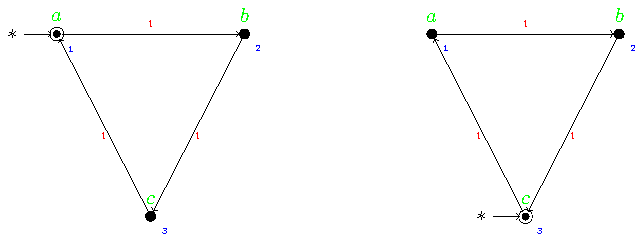
\includegraphics[scale=.8]{images/counterexample.pdf}
	\caption{Two TGs, $Q$ (left) and $R$ (right), having a different set of traces but the same embedding representation.}\label{fig:counterexample}
\end{figure}
\begin{proposition}\label{lem:rewritinglemma}
Given two TGs $P=(s,t,L,R,w)$ and $P'=(s',t',L',R',w')$, the TG Kernel is defined as follows:
$$\begin{aligned}
k_{\phi_{\mathcal{P}}}(P,P')=&ww't_f^{|R>0|+|R'>0|}\left(1-\frac{\norm{\hat{\epsilon}-\hat{\epsilon}'}{2}^2}{2}\right)+\\
	&+t_f^{|R>0|+|R'>0|}\left(1-\frac{\norm{\hat{\nu}-\hat{\nu}'}{2}^2}{2}\right)\\
\end{aligned}$$
\end{proposition}
\begin{proof}
$$\begin{aligned}
k_{\phi_{\mathcal{P}}}(P,P')&=\Braket{\phi_{\mathcal{P}}(P),\phi_{\mathcal{P}}(P')}\\
	&=\sum_{\alpha\beta\in \Sigma_\varepsilon^2}\frac{\epsilon_{\color{green}\alpha\beta}}{\|\epsilon\|_2}\frac{{\epsilon'}_{\color{green}\alpha\beta}}{\|\epsilon'\|_2}ww't_f^{|R>0|+|R'>0|}\quad+\quad \sum_{\alpha\in \Sigma_\varepsilon}\frac{\nu_{\color{green}\alpha}}{\|\nu\|_2}\frac{{\nu'}_{\color{green}\alpha}}{\|\nu'\|_2}t_f^{|R>0|+|R'>0|}\\
	&=ww'\tau^{|Rb>0|+|R'>0|}\sum_{\alpha\beta\in \Sigma_\varepsilon^2}\frac{\epsilon_{\color{green}\alpha\beta}}{\|\epsilon\|_2}\frac{{\epsilon'}_{\color{green}\alpha\beta}}{\|\epsilon'\|_2}\quad+\quad t_f^{|R>0|+|R'>0|}\sum_{\alpha\in \Sigma_\varepsilon}\frac{\nu_{\color{green}\alpha}}{\|\nu\|_2}\frac{{\nu'}_{\color{green}\alpha}}{\|\nu'\|_2}\\
	&=ww't_f^{|R>0|+|R'>0|}\Braket{\hat{\epsilon}, \hat{\epsilon}'}+ t_f^{|R>0|+|R'>0|}\Braket{\hat{\nu}, \hat{\nu}'}\\
	&=ww't_f^{|R>0|+|R'>0|}\left(1-\frac{\norm{\hat{\epsilon}- \hat{\epsilon}'}{2}^2}{2}\right)+ t_f^{|R>0|+|R'>0|}\left(1-\frac{\norm{\hat{\nu}- \hat{\nu}'}{2}^2}{2}\right)\\
\end{aligned}$$
\end{proof}

\subsection{Properties}
As a first property, we want to show that when the two TGs are (trace) equivalent, then there exists an embedding configuration for which the kernel computation reduces to the two TGs' weight product, i.e. $ww'$. The kernel will then represent the probability that both Petri Nets are valid contemporaneously and, when both weights are $1$, the kernel returns $1$. We will call this condition  ``weak equality'' because we cannot possibly prove that $k_{\phi_{\mathcal{P}}}(P,P')=ww'\Leftrightarrow \mathcal{W}_p^n(P)=\mathcal{W}_p^n(P')$, as there could be similar embeddings coming from Petri Nets sharing a different weighted traces set ($\mathcal{W}_p^n(P)\neq\mathcal{W}_p^n(P')$).

\begin{example}
	If we use $\epsilon$ and $\nu$ as defined in Equations \ref{eq:epsilon}-\ref{eq:nu}, we might have a false positive for ``weak equality'' if $Q=(s,s,L,R,w)$ and $R=(s',s',L,R,w)$ are both cycle graphs with $s\neq s'$, $\textit{label}(s)\neq\textit{label}(s')$, $\textit{label}(s)\neq\varepsilon$, and $\textit{label}(s')\neq\varepsilon$. An intuitive example of such situation is presented in Figure \ref{fig:counterexample}: both graphs will have the same frequency for both subtraces and nodes, and therefore have the same  $\epsilon$ and $\nu$ by construction. By having different initial and accepting node with  different labels, we have $\mathcal{W}_0^{\aleph_0}(Q)=\Set{\textup{a(bca)}^n|n\in\mathbb{N}}$ and $\mathcal{W}_0^{\aleph_0}(R)=\Set{\textup{c(abc)}^n|n\in\mathbb{N}}$, thus implying $\mathcal{W}_0^{\aleph_0}(Q)\neq\mathcal{W}_0^{\aleph_0}(R)$ but $k_{\phi_{\mathcal{P}}}(Q,R)=1$ for $t_f=1$.
\end{example}


\begin{lemma}[Weak Equality]
Given two TGs $P=(s,t,L,R,w)$ and $P'=(s',t',L',R',w')$ providing the same set of weighted traces, then $k_{\phi_{\mathcal{P}}}(P,P')=ww'$ for $t_f=1$.
\end{lemma}
\begin{proof}
Given Proposition \ref{lem:rewritinglemma} and the positive definition of $\epsilon$ and $\nu$,  we have that $\norm{\hat{\epsilon}-\hat{\epsilon}'}{2}\to 0$ as well as $\norm{\hat{\nu}-\hat{\nu}'}{2}\to 0$, for which we can immediately close the goal.
\end{proof}

As per previous observations, we know that two TGs should have the maximum dissimilarity when all the non $\varepsilon$-nodes have different labels, thus making it impossible to find an alignment, thus implying that they share an utterly dissimilar set of weighted traces.

\begin{lemma}[Strong Dissimilarity]
Given two TGs $P=(s,t,L,R,w)$ and $P'=(s',t',L',R',w')$, $k_{\phi_{\mathcal{P}}}(P,P')=0$ iff. $P$ and $P'$ have a different set of labels with $t_f,w,w'>0$.
\end{lemma}
\begin{proof}
If we exclude the trivial conditions $t_f=0$, $w=0$ or $w'=0$, the only condition when the kernel returns zero is when  $\Braket{\hat{\epsilon},\hat{\epsilon}'}=0$ and $\Braket{\hat{\nu},\hat{\nu}'}=0$. This implies that, when a component of $\epsilon$ (or $\nu$) is non-zero, the same component of $\epsilon'$ (or $\nu'$) is zero and viceversa. This directly requires that there is a different set of labels associated to the nodes. 
\end{proof}

As a corollary of the two lemmas, we have that the proposed embedding performs weakly-ideally, as the equality condition holds only on a relaxed form.

Last, under the assumption that a TG is approximately characterized by $\epsilon$ and $\nu$, we might expect that the TG similarity is characterized by the sum of the distance of both embeddings. Therefore, we show that an increase in both distance embeddings approximately corresponds to a decrease in the kernel output and vice-versa.\yellownote{TODO (if required), establish the further approximation from such distributions and the actual expected ranking.}

\begin{lemma}\label{lem:approxRank}
Given two TGs $P=(s,t,L,R,w)$ and $P'=(s',t',L',R',w')$ having respectively the embeddings $(\epsilon,\nu)$ and $(\epsilon',\nu')$, we have that the kernel $k_{\phi_{\mathcal{T}}}$ induces an inverse ranking of $\norm{\hat{\epsilon}-\hat{\epsilon}'}{2}+\norm{\hat{\nu}-\hat{\nu}'}{2}$:
$$k_{\phi_{\mathcal{T}}}(P,P')\appropto 2-(\norm{\hat{\epsilon}-\hat{\epsilon}'}{2}+\norm{\hat{\nu}-\hat{\nu}'}{2})$$
\end{lemma}
\begin{proof}
Let us use $T=t_f^{|R>0|+|R'>0|}$, $\omega=ww'$, $V=\norm{\hat{\nu}-\hat{\nu}'}{2}$, and $E=\norm{\hat{\epsilon}-\hat{\epsilon}'}{2}$ as shorthands. The goal can be rewritten as $k_{\phi_{\mathcal{T}}}(P,P')\appropto 2-(E+V)$. Given that the embeddings $(\epsilon,\nu)$ and $(\epsilon',\nu')$ are normalized kernel function $k_{\phi_{\mathcal{P}}}$ and that they are always positive definite, then we have that $0\leq E +V\leq 2$, so $0\leq 2-(E+V)\leq 2$. Using Proposition \ref{lem:rewritinglemma}, we can write $k_{\phi_{\mathcal{P}}}(P,P')$ as follows:
$$\left(1-\frac{E}{2}\right)\omega T+\left(1-\frac{V}{2}\right)T=T\left(\omega+1-\frac{E\omega+V}{2}\right)$$
Given that the embeddings $(\epsilon,\nu)$ and $(\epsilon',\nu')$ are normalized in $k$ and that they are always positive definite,  we also have that $0\leq E\omega +V\leq 2$ where $0\leq \omega\leq 1$. We can also write  $0\leq \omega+1-\frac{E\omega+V}{2}\leq \frac{2}{T}$. For $\omega,T=1$, we have that $k_{\phi_{\mathcal{P}}}(P,P')=2-\frac{(E+V)}{2}$. Thus, $0<\omega,T<1$ approximates the expected ranking. 
\end{proof}

Given that we can now follow Definition \ref{def:ppne} for representing a trace $\tau$ as a proper embedding after transforming it as a TG $T$ (\S\ref{subsec:katk}), we can find the TG $P$ providing the best approximate match with  a trace $\tau$ as follows:
\[\underset{{P}}{\max\arg}\;k_{\phi_{\mathcal{P}}}(P,T)\]
Still, this TG matching strategy does not allow to find the trace maximizing such score. To assess such problem, the next section is going to determine both an exact (\S\ref{subsec:exbkptap}) and an approximated strategy (\S\ref{subsec:akptap}) for probabilistically matching one single trace from the TG.

